%% This is an example first chapter.  You should put chapter/appendix that you
%% write into a separate file, and add a line \include{yourfilename} to
%% main.tex, where `yourfilename.tex' is the name of the chapter/appendix file.
%% You can process specific files by typing their names in at the 
%% \files=
%% prompt when you run the file main.tex through LaTeX.
\chapter{Testing}

\section{Unit Testing}

\section{Performance Testing}

Performance testing comprehends any process of determining the quality attributes of a system such as responsiveness, stability and reliability under certain workloads. It is usually used to verify that the system meets its specifications.

Load testing is the simplest form of performance testing. Load tests are conducted to assess the behaviour of the system under a particular load. The load is defined by a particular number of transactions and a certain level of concurrency within a specified duration. In the context of a web system the transactions are round trip of HTTP requests to a particular endpoint and the concurrency level is the number of requests performed at a time. As a result, the test outputs the response times of these requests and may uncover bottlenecks of the system.

There are numerous variables involved in the execution of the system such as network reliability, performance of the underlying hardware, availability of third-party services, etc. Therefore, the following load test does not aim to give the exact performance of the system, but its approximate behaviour under conditions similar to a real scenarios making some reasonable assumptions.

The tests have been conducted using two simple yet powerful and mature open-source tools: Apache Bench and Gnuplot. Apache Bench is a server benchmarking tool that focuses on showing how many requests per second a system is able to serve. It provides basic statistic functions such as mean, median, minimum and maximum of the measured magnitudes. Gnuplot, on the other hand, makes it easy to draw charts from diverse input text formats by means of a scripting language or interactive console.

As the system has two entry points, the one used by the sensors and the web application, two different load test have been performed. By doing so, we can assess the performance of the Sensor Observation Service and the Web application.

TODO what about the queue??

\subsection{Web Application}

First and foremost, the variables involved in determining the response times of the requests must be defined. These are concurrency and number of requests per test.

\paragraph{Concurrency} We distinguish two different levels of concurrency. First, when a browser loads a web page it starts multiple connection to the server to load the resources. The number of simultaneous connections is a built-in browser parameter that for most of the web browsers defaults to 6. Besides, concurrency in a load testing often refers to the number of users issuing requests to the system at a time. The increases in this variable define the number of executions of the test.

\paragraph{Number of requests} This is the total number of requests issued to the system for each execution of the test. However, each time a user loads a web page the browser makes as many requests as assets the page contains. That is, the browser loads each of the CSS files, images and JS scripts the HTML states, one per request.

The single HTML page of the application contains 46 assets, loading 717 KB of data. These resources contain the JS application sources plus the map tiles and other resources fetched by the map client. Moreover, as the user interacts with the map, more tiles are loaded by the browser. Nevertheless, these requests don't hit our system, but the Mapbox's servers. Hence, they are not taken into account, although they impact on the perceived performance of the system. The size of each resource is assumed to be the average, 717 KB / 46 resources = 15,6 KB.

\subsubsection*{Baseline}

To serve as comparison the baseline is defined as a test with a single request to load the HTML page followed by 46 request with 6 concurrent connections to load the assets of 15,6 KB each. This tries to mimic the behaviour while simplifying the intricacies of the browser concurrency and assuming the content is instantly rendered.

\begin{listing}[h]
\begin{minted}[
baselinestretch=1.2,
fontsize=\footnotesize
] {bash}
(...)

Document Path:          /test_asset
Document Length:        15600 bytes

Concurrency Level:      6
Time taken for tests:   1.845 seconds
Complete requests:      46
Failed requests:        0
Keep-Alive requests:    46
Total transferred:      729330 bytes
HTML transferred:       717600 bytes
Requests per second:    24.94 [#/sec] (mean)
Time per request:       240.603 [ms] (mean)
Time per request:       40.100 [ms] (mean, across all concurrent requests)
Transfer rate:          386.12 [Kbytes/sec] received

Connection Times (ms)
              min  mean[+/-sd] median   max
Connect:        0    8  19.9      0      64
Processing:    87  223 241.9    142    1448
Waiting:       54  110  26.9     99     189
Total:         87  231 249.4    142    1448

Percentage of the requests served within a certain time (ms)
  50%    142
  66%    159
  75%    259
  80%    265
  90%    378
  95%    748
  98%   1448
  99%   1448
 100%   1448 (longest request)
\end{minted}
\label{fig:baseline}
\caption{Output of the command \texttt{ab} for the baseline}
\end{listing}

As shown in \ref{fig:baseline}, the application assets are loaded in 231ms at 396KB/s. Together with the response time of a single request, this means a user waits $231ms + 431ms = 662ms$ seconds by average until the whole application is fully loaded.

\subsubsection*{10 Users Scenario}

In the following test executions the concurrency is increased progressively in order to simulate more demanding scenarios. First, simulating 10 users and then 50. For each of these, half of the required requests point to the HTML and the other half to the assets, thereby, simulating requests that impact the server differently.

Therefore, the first test issues 10 concurrent requests to load the HTML, while 460 more requests with 60 concurrent connections load the assets.

\begin{listing}[h]
\begin{minted}[
baselinestretch=1.2,
fontsize=\footnotesize
] {bash}
(...)

Document Path:          /
Document Length:        2406 bytes

Concurrency Level:      10
Time taken for tests:   2.967 seconds
Complete requests:      10
Failed requests:        0
Keep-Alive requests:    10
Total transferred:      27460 bytes
HTML transferred:       24060 bytes
Requests per second:    3.37 [#/sec] (mean)
Time per request:       2966.874 [ms] (mean)
Time per request:       296.687 [ms] (mean, across all concurrent requests)
Transfer rate:          9.04 [Kbytes/sec] received

Connection Times (ms)
              min  mean[+/-sd] median   max
Connect:      100  106   2.9    107     110
Processing:   241  529 821.4    276    2867
Waiting:      236  380 370.9    270    1435
Total:        345  636 819.3    383    2967

Percentage of the requests served within a certain time (ms)
  50%    383
  66%    390
  75%    397
  80%    404
  90%   2967
  95%   2967
  98%   2967
  99%   2967
 100%   2967 (longest request)
 \end{minted}
\label{fig:kn10c10}
\caption{Output of the command \texttt{ab} with 10 concurrent connections}
\end{listing}

\begin{listing}[h]
\begin{minted}[
baselinestretch=1.2,
fontsize=\footnotesize
] {bash}
(...)

Document Path:          /test_asset
Document Length:        15600 bytes

Concurrency Level:      60
Time taken for tests:   33.881 seconds
Complete requests:      460
Failed requests:        0
Keep-Alive requests:    460
Total transferred:      7293300 bytes
HTML transferred:       7176000 bytes
Requests per second:    13.58 [#/sec] (mean)
Time per request:       4419.294 [ms] (mean)
Time per request:       73.655 [ms] (mean, across all concurrent requests)
Transfer rate:          210.22 [Kbytes/sec] received

Connection Times (ms)
              min  mean[+/-sd] median   max
Connect:        0   17  48.0      0     212
Processing:   401 2677 2836.6   1979   31183
Waiting:       71  431 699.3    217    7835
Total:        401 2695 2849.7   1993   31183

Percentage of the requests served within a certain time (ms)
  50%   1993
  66%   2608
  75%   3115
  80%   3535
  90%   4596
  95%   7347
  98%  11424
  99%  18008
 100%  31183 (longest request)
 \end{minted}
\label{fig:kn460c60}
\caption{Output of 460 requests with 60 concurrent connections}
\end{listing}

All users' browser loaded the application in $2695ms + 636ms = 3331ms$ in average. However, the standard deviation turns out to be remarkably high. The resulting values shown in \ref{fig:kn460c60} are summarized in the chart \ref{fig:kn460c60_chart}.

\begin{sidewaysfigure}[h]
	\centering
	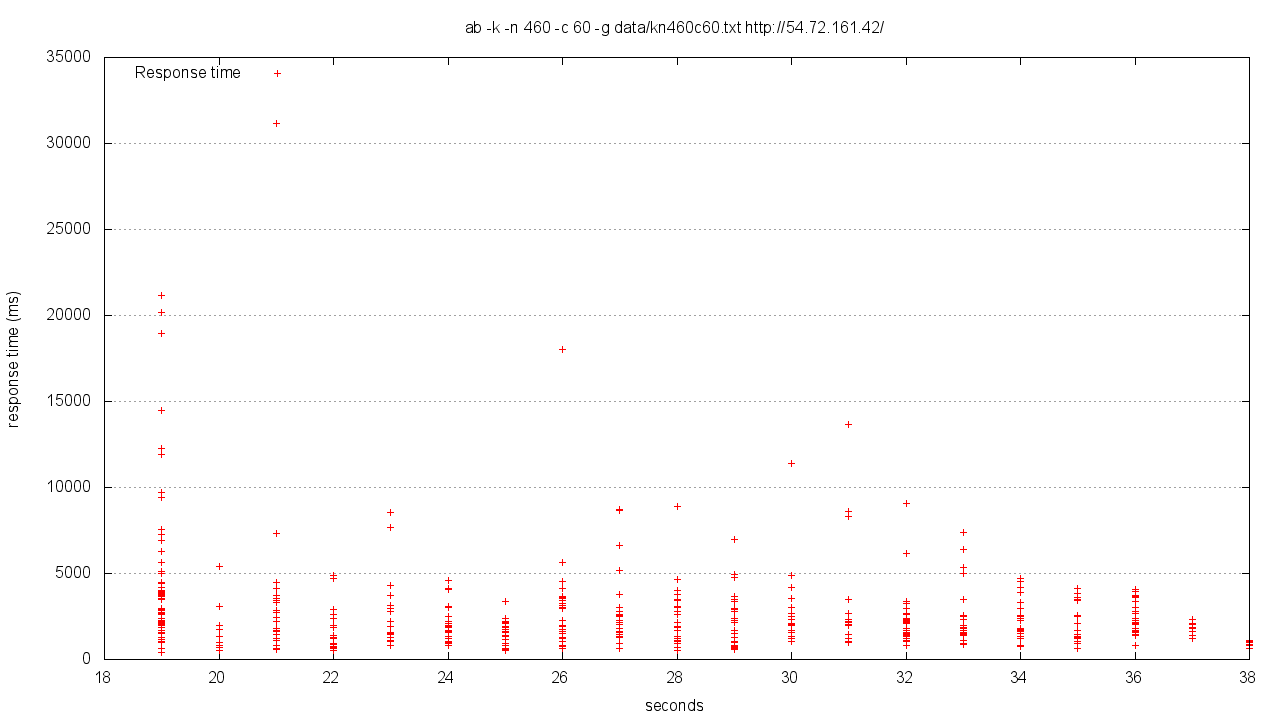
\includegraphics[width=\textwidth]{kn460c60}
	\caption{Response time plot of 460 requests with 60 concurrent connections}
	\label{fig:kn460c60_chart}
\end{sidewaysfigure}

\subsubsection*{30 Users Scenario}

To test the load equivalent to 30 users this execution sends 30 concurrent requests plus 1380 requests with 180 concurrent connections.

\begin{listing}[h]
\begin{minted}[
baselinestretch=1.2,
fontsize=\footnotesize
] {bash}
(...)

Document Path:          /
Document Length:        2406 bytes

Concurrency Level:      30
Time taken for tests:   1.607 seconds
Complete requests:      30
Failed requests:        0
Keep-Alive requests:    30
Total transferred:      82380 bytes
HTML transferred:       72180 bytes
Requests per second:    18.67 [#/sec] (mean)
Time per request:       1606.587 [ms] (mean)
Time per request:       53.553 [ms] (mean, across all concurrent requests)
Transfer rate:          50.07 [Kbytes/sec] received

Connection Times (ms)
              min  mean[+/-sd] median   max
Connect:      240  260  10.9    266     279
Processing:   350  752 443.5    457    1356
Waiting:      347  747 444.8    453    1354
Total:        600 1013 437.1    726    1606

Percentage of the requests served within a certain time (ms)
  50%    726
  66%   1555
  75%   1561
  80%   1572
  90%   1602
  95%   1604
  98%   1606
  99%   1606
 100%   1606 (longest request)
 \end{minted}
\label{fig:kn30c30}
\caption{Output of 30 concurrent connections}
\end{listing}

\begin{listing}[h]
\begin{minted}[
baselinestretch=1.2,
fontsize=\footnotesize
] {bash}
(...)

Document Path:          /test_asset
Document Length:        15600 bytes

Concurrency Level:      180
Time taken for tests:   102.233 seconds
Complete requests:      1380
Failed requests:        54
   (Connect: 0, Receive: 0, Length: 54, Exceptions: 0)
Keep-Alive requests:    1326
Total transferred:      21187354 bytes
HTML transferred:       20841574 bytes
Requests per second:    13.50 [#/sec] (mean)
Time per request:       13334.721 [ms] (mean)
Time per request:       74.082 [ms] (mean, across all concurrent requests)
Transfer rate:          202.39 [Kbytes/sec] received

Connection Times (ms)
              min  mean[+/-sd] median   max
Connect:        0  128 652.6      0    4900
Processing:     0 6618 17501.4    831   95570
Waiting:       54 1260 6032.2    193   49972
Total:          0 6745 17697.4    843   97127

Percentage of the requests served within a certain time (ms)
  50%    843
  66%   1348
  75%   1843
  80%   2547
  90%  21964
  95%  45340
  98%  86613
  99%  91950
 100%  97127 (longest request)
 \end{minted}
\label{fig:kn1380c180}
\caption{Output of 1380 requests with 180 concurrent connections}
\end{listing}

\begin{sidewaysfigure}[h]
	\centering
	\includegraphics[width=\textwidth]{kn1380c180}
	\caption{Response time plot of 1380 requests with 180 concurrent connections}
	\label{fig:kn2300c300_chart}
\end{sidewaysfigure}

- Some failed requests
- Throughput kept around 13.5 req/sec. It didn't partially because of the failures.
- Something is wrong when stdev is more than 2 times the mean.
- Poor reliability

\section{Sensor Observation Service}

This test aims to test the performance of system while receiving requests from the sensors. This test impacts on the SOS and the database, hence the bottleneck is likely to be one of this components. In contrast with previous load test, since SOS is essentially a set of HTTP endpoints regular requests with an increasing level of concurrency are enough to assess the performance of the system.

Nevertheless, the requirements state that sensors are required to perform only a request every 10 minutes, resulting in 6 requests per hour. If higher resolution was required requests would also be evenly distributed. Thus, the test must take into account this time spans.

\subsection{Baseline}

For this test the baseline is defined as a single POST request to each of the two endpoints: /sensors and /observations. Both have fairly similar behaviour, processing the request and storing results in the database, and receive payloads of similar size. Hence, there is no need for combining these request as it does not provide any valuable insight. The results of both executions are shown in \ref{fig:sensors_n1c1} \ref{fig:observations_n1c1}.

\begin{listing}[h]
\begin{minted}[
baselinestretch=1.2,
fontsize=\footnotesize
] {bash}
(...)

Document Path:          /webapp/sos/rest/sensors
Document Length:        890 bytes

Concurrency Level:      1
Time taken for tests:   0.511 seconds
Complete requests:      1
Failed requests:        0
Total transferred:      1210 bytes
Total body sent:        3003
HTML transferred:       890 bytes
Requests per second:    1.96 [#/sec] (mean)
Time per request:       510.607 [ms] (mean)
Time per request:       510.607 [ms] (mean, across all concurrent requests)
Transfer rate:          2.31 [Kbytes/sec] received
                        5.74 kb/s sent
                        8.06 kb/s total

Connection Times (ms)
              min  mean[+/-sd] median   max
Connect:       48   48   0.0     48      48
Processing:   463  463   0.0    463     463
Waiting:      462  462   0.0    462     462
Total:        511  511   0.0    511     511
 \end{minted}
\label{fig:sensors_n1c1}
\caption{Output of a POST request to /sensors}
\end{listing}

\begin{listing}[h]
\begin{minted}[
baselinestretch=1.2,
fontsize=\footnotesize
] {bash}
(...)

Document Path:          /webapp/sos/rest/observations
Document Length:        854 bytes

Concurrency Level:      1
Time taken for tests:   0.655 seconds
Complete requests:      1
Failed requests:        0
Total transferred:      1210 bytes
Total body sent:        2204
HTML transferred:       854 bytes
Requests per second:    1.53 [#/sec] (mean)
Time per request:       654.535 [ms] (mean)
Time per request:       654.535 [ms] (mean, across all concurrent requests)
Transfer rate:          1.81 [Kbytes/sec] received
                        3.29 kb/s sent
                        5.09 kb/s total

Connection Times (ms)
              min  mean[+/-sd] median   max
Connect:       59   59   0.0     59      59
Processing:   595  595   0.0    595     595
Waiting:      592  592   0.0    592     592
Total:        654  654   0.0    654     654
 \end{minted}
\label{fig:observations_n1c1}
\caption{Output of a POST request to /observations}
\end{listing}

\subsubsection*{First scenario}

In this scenario the load is compound of 10 sensors sending observations every minute concurrently. Thus, the resolution of the observations increases up until 60 observations per hour.

